%%%%%%%%%%%%%%%%%%%%%%%%%%%%%%%%%%%%%%%%%%%%%%%%%%%%%%%%%%%%%%%%%%%%%%%%%%%%%%%
%  Coursework template                                                        %
%  Advanced Control Systems lecture, RWTH Aachen University                   %
%  Version 1.01, 2014                                                         %
%%%%%%%%%%%%%%%%%%%%%%%%%%%%%%%%%%%%%%%%%%%%%%%%%%%%%%%%%%%%%%%%%%%%%%%%%%%%%%%

\documentclass{scrreprt}

%%%%%%%%%%%%%%%%% Please fill in the correct information here %%%%%%%%%%%%%%%%%    

%% Uncomment the right topic
\title{Multivariable Control Problems}
%\title{Multivariable Control Problems}
%\title{Quadruple Tank}

\author{Raj Khamkar}

%% Leave commented to print current date
\date{25.02.2023} 

%%%%%%%%%%%%%%%%%%%%%%%%%%%% Include packages here %%%%%%%%%%%%%%%%%%%%%%%%%%%% 

\usepackage{amsmath,bm}
\usepackage{array}
\usepackage{color}
\usepackage{fancyhdr}
\usepackage{graphicx}
\usepackage{listings}
\usepackage{pgfplots}
\usepackage{siunitx}
\usepackage{tikz}
\usetikzlibrary{arrows,shapes,backgrounds,positioning,plotmarks}
\usepackage{titlesec}
\usepackage{url}

%%%%%%%%%%%%%%%%%%%%%%%%%%% DO NOT MODIFY THIS PART %%%%%%%%%%%%%%%%%%%%%%%%%%%

\subtitle{Coursework}
\makeatletter
\let\runauthor\@author
\let\runtitle\@title
\makeatother

\newcommand{\taskapp}{Task}
\renewcommand*\chapterformat{\taskapp~\thechapter:~}

\titleformat{\section}{\large\bfseries}{}{0pt}{Question \thesection:~}

\fancypagestyle{plain}{
  \fancyhf{}
  \fancyhead[C]{\runtitle}
	\fancyhead[R]{\thepage}
	\fancyhead[L]{\runauthor}
}

\begin{document}

%% Titlepage
\maketitle

%% Table of contents
\tableofcontents 

\cleardoublepage

\pagestyle{plain}

%%%%%%%%%%%%%%%%%%%%%%%%%%%%% Content starts here %%%%%%%%%%%%%%%%%%%%%%%%%%%%%

%\chapter{Brief Info}
%This report can be written in English or German, it should have a similar organisation to the problem description. Please be as brief and precise as possible, reports with more than 30 pages will be rejected.
%
%\section{Formulas and equations}
%Please use labels to refer to your equations, like in Eq.~\eqref{eq:T}:
%\begin{equation}
%  T(s) = \frac{3001 \: (1 + 0.3343s)}{s^3 + 3 s^2 + 3s + 1} \text{.}
%  \label{eq:T}
%\end{equation}
%Equations do not relieve you from the use of punctuation marks. Feel free to align long equations like the next one (without numbering, hence the asterisk)
%\begin{align*}
%  T(s) &= \frac{\frac{K_i}{m s^2 - K_x} \: K_R \: \frac{1 + s \tau_1}{1 + s \tau_2}}
%          {1 + \frac{K_i}{m s^2 - K_x} \: K_R \: \frac{1 + s \tau_1}{1 + s \tau_2}} \\
%       &= \frac{K_i K_R (1 + s \tau_1)}{(m s^2 - K_x) (1 + s \tau_2) + K_i K_R (1 + s \tau_1)} \\
%       &= \frac{K_i K_R (1 + s \tau_1)}
%          {m \tau_2 s^3 + m s^2 + (\tau_1 K_i K_R - \tau_2 K_x) s + K_i K_R - K_x} \\
%       &= \frac{K_i K_R \: \frac{1 + s \tau_1}{m \tau_2}}
%          {s^3 + \frac{1}{\tau_2} s^2 + \frac{\tau_1 K_i K_R - \tau_2 K_x}{m \tau_2} s 
%          + \frac{K_i K_R - K_x}{m \tau_2}} \text{.}
%\end{align*} 
%If you use indices like $x$ in $A_x$, please define them as text if they are not variables like in $A_\text{Beer}$. Note that $A_{Beer}$ would be wrong. Stick to the notation from~\cite{Sko05} or the lecture notes as far as possible. Matrices and vectors should be bold faced, for example $\mathbf{A}$ or $\mathbf{u}$. Please use the siunitx package for adding SI units to numerical values, example \SI[per-mode=fraction]{5}{\meter\per\second}.
%
%\section{Figures}
%Please add figures in a floating figure environment as shown in Fig.~\ref{fig:superC}.
%\begin{figure}[htb]
%  \centering
%  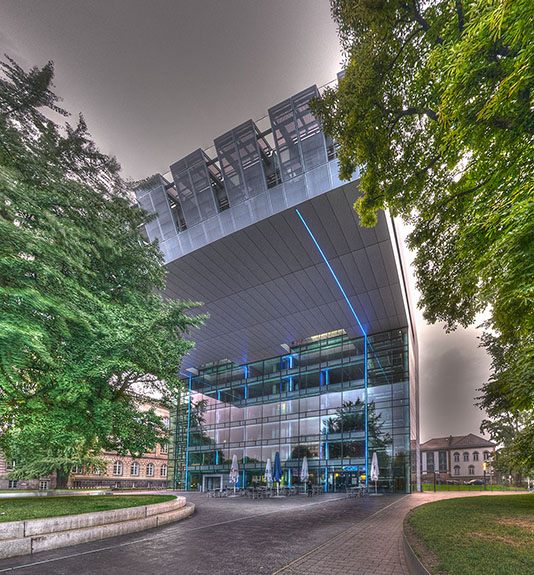
\includegraphics[scale=0.5]{images/superC}
%  \caption{Nice picture of the big bus stop.}
%  \label{fig:superC}
%\end{figure}
%Figures should be not wider than the attribute textwidth, starting with a backslash. Please note the full stop at the end of the caption of the figure. And note that the figure floats away, a nice explanation from Wikipedia: Floats are not part of the normal stream of text, but separate entities, positioned in a part of the page to themselves (top, middle, bottom, left, right, or wherever the designer specifies). They always have a caption describing them and they are always numbered so they can be referred to from elsewhere in the text. LaTeX automatically floats Tables and Figures, depending on how much space is left on the page at the point that they are processed. If there is not enough room on the current page, the float is moved to the top of the next page. This can be changed by moving the Table or Figure definition to an earlier or later point in the text, or by adjusting some of the parameters which control automatic floating.
%
%\section{Block diagrams}
%A cool way to create block diagrams is tikz, an example is depicted in Fig.~\ref{fig:blockDiagram}.
%\begin{figure}[htb]
%  \centering
%  \tikzstyle{block}     = [draw, rectangle, minimum height=1cm, minimum width=1.6cm]
%    \tikzstyle{branch}    = [circle, inner sep=0pt, minimum size=1mm, fill=black, draw=black]
%    \tikzstyle{connector} = [->, thick]
%    \tikzstyle{dummy}     = [inner sep=0pt, minimum size=0pt]
%    \tikzstyle{inout}     = []
%    \tikzstyle{sum}       = [circle, inner sep=0pt, minimum size=2mm, draw=black, thick]
%    \begin{tikzpicture}[auto, node distance=1.6cm, >=stealth']
%      \node[block] (K) {$\mathbf{K}$};
%      \node[block] (G) [right=of K] {$\mathbf{G}$};
%      \node[sum] (s1) [left=of K] {};
%      \node[inout] (r) [left=of s1] {$\mathbf{r}$};
%      \node[sum] (s2) [right=of G] {};
%			\node[block] (Gd) [above=0.6cm of s2] {$\mathbf{G}_d$};
%      \node[inout] (d) [above=0.6cm of Gd] {$\mathbf{d}$};  
%      \node[branch] (b1) [right=of s2] {};
%      \node[inout] (y) [right=of b1] {$\mathbf{y}$};
%      \node[sum] (s3) [below=0.8cm of b1] {};
%      \node[inout] (n) [right=of s3] {$\mathbf{n}$};
%      \node[dummy] (d1) [below right=0.1cm and 0.05cm of s1] {$-$};
%        
%      \draw[connector] (s1) -- (K);
%      \draw[connector] (K) -- node {$\mathbf{u}$} (G);
%      \draw[connector] (G) -- (s2);
%      \draw[thick] (s2) -- (b1);
%      \draw[connector] (b1) -- (y);
%      \draw[connector] (b1) -- (s3);
%      \draw[connector] (n) -- (s3);
%      \draw[connector] (d) -- (Gd);
%      \draw[connector] (Gd) -- (s2);
%      \draw[connector] (r) -- (s1);
%      \draw[connector] (s3) -| node [yshift=0.3cm] {$\mathbf{y}_m$} (s1);
%    \end{tikzpicture}
%	  \caption{One degree-of-freedom feedback control system.}
%    \label{fig:blockDiagram}
%\end{figure}
%
%\chapter{More Info}
%There should always be some text between the chapter title and your first section.
%
%\section{Figure export from Matlab}
%There is a nice way to export figures from matlab to tikz, check \url{http://www.mathworks.com/matlabcentral/fileexchange/22022-matlab2tikz-matlab2tikz}. An example of a bar plot with pgfplots looks like Fig.~\ref{fig:barPlot}.
%
%\begin{figure}[!tb]
%  \centering
%  \begin{tikzpicture}
%    \pgfplotsset{compat=1.3}
%    \begin{axis}[
%      width=0.8\textwidth,
%      xtick = data,
%      symbolic x coords={ {Beer}, {Cocktails}, {Shots}, {Wine} },
%      ymin = 0, ymax = 22,
%      ylabel = { Flow rate $\left[ \si[per-mode=fraction]{\milli\liter\per\hour} \right]$ },
%      legend style={ at={(0.5,-0.12)},
%      anchor=north, legend columns=-1
%      font=\tiny},
%      ybar=5pt,
%      bar width = 20pt,
%      ymajorgrids = true
%      ]
%      
%      \addplot coordinates { (Beer,20.66) (Cocktails,9.86) (Shots,18.62) (Wine,21.87) };
%      \addplot coordinates { (Beer,15.3) (Cocktails,9.827) (Shots,17.77) (Wine,19.41) };     
%           
%      \addplot[ green!60!black ,sharp plot,update limits=false ] coordinates {(Beer,4.22) (Wine,4.22)};
%      \draw[ green!60!black, thick ] ({rel axis cs:0,0}|-{axis cs:Wine,4.22}) -- ({rel axis cs:1,0}|-{axis cs:Wine,4.22});
%
%      \legend{ {Good party \qquad}, 
%               {Mediocre party \quad},
%               Minimum}
%      
%    \end{axis}
%  \end{tikzpicture}
%  \label{fig:barPlot}
%  \caption{Do not try this at home.}
%\end{figure}

\chapter{System Analysis}

\section{Spectral decomposition}
The transfer funtion of a state-space system $\mathbf{G(s)}$, can be expressed as equation~\eqref{eq:T},
\begin{equation}
 \bm{G(s)} = \bm{C} \: (s\bm{I} - \bm{A})^{-1} \: \bm{B} + \bm{D} \text{.}
  \label{eq:T}
\end{equation}
where $\bm{A}, \bm{B}, \bm{C}, \bm{D}$  are matrices in the minimum realization. $\bm{A}$  has no repeated eigenvalues and is symmetric. In order to decompose this transer function~\eqref{eq:T} into its dyadic expansion~\eqref{eq:D},
\begin{equation}
 \bm{G(s)} = \sum_{i=1}^n \frac{\bm{y}_{pi}\: \bm{u}_{pi}^H}{s - p_i} + \bm{D} \text{.}
  \label{eq:D}
\end{equation}
with given pole vectors;
\begin{equation}
 \bm{G(s)} = \sum_{i=1}^n \frac{\bm{C}\: \bm{t}_i\: \bm{q}_i^H\: \bm{B}}{s - \lambda_i} + \bm{D} \text{.}
  \label{eq:D1}
\end{equation}
From the Shift theorem we know that the eigenvalues of (s$\bm{I} - \bm{A}$) are equal to the eigenvalues of (s - $\lambda_i$)
and that the eigenvectors of  (s$\bm{I} - \bm{A}$) are equal to the eigenvectors of $\bm{A}$.
Expanding dyadically; 
\begin{align*}
\bm{A} &= \sum_{i=1}^n \lambda_i \: \bm{t}_i\: \bm{q}_i^H \\
s\bm{I} - \bm{A} &= \sum_{i=1}^n (s - \lambda_i) \: \bm{t}_i\: \bm{q}_i^H \\
\end{align*}
Assuming a matrix $\bm{T}$ contains the eigenvectors of (s$\bm{I} - \bm{A}$) as columns, we can solve for eigenvectors of (s$\bm{I} - \bm{A})^{-1}$ as follows:
\begin{align*}
\bm{T}^{-1}\: (s\bm{I} - \bm{A})^{-1}\: \bm{T} &= \bm{\Lambda}^{-1} \\
	&= (\bm{T}^{-1}\: (s\bm{I} - \bm{A})\: \bm{T})^{-1} \\
\end{align*}
Using the Shifting Theorem:
\begin{align*}
\bm{T}^{-1}\: (s\bm{I} - \bm{A})\: \bm{T} &=  s\bm{I} - \bm{\Lambda} \\
\bm{T}^{-1}\: (s\bm{I} - \bm{A})^{-1}\: \bm{T} &= (s\bm{I} - \bm{\Lambda})^{-1} \\
\end{align*}
\begin{align*}
(s\bm{I} - \bm{A})^{-1} &= \sum_{i=1}^n \lambda_i\: (s\bm{I} - \bm{A})\: \bm{t}_i\: \bm{q}_i^H \\
	&= \sum_{i=1}^n \frac{\bm{t}_i\: \bm{q}_i^H}{(s - \lambda_i)}
\end{align*}
\begin{align*}
\bm{G(s)} &=  \bm{C} \: (s\bm{I} - \bm{A})^{-1} \: \bm{B} + \bm{D} \\
	&= \bm{C}\: \sum_{i=1}^n \frac{\bm{t}_i\: \bm{q}_i^H}{(s - \lambda_i)}\: \bm{B} + \bm{D} \\
	&= \sum_{i=1}^n \frac{\bm{C}\: \bm{t}_i\: \bm{q}_i^H\: \bm{B}}{s - \lambda_i} + \bm{D} \\
\end{align*}
hence proven,
\begin{equation}
\bm{G(s)} = \sum_{i=1}^n \frac{\bm{y}_{pi}\: \bm{u}_{pi}^H}{s - \lambda_i} + \bm{D} \text{.}
\end{equation}
Testing for a random plant $\bm{A}$: 
\begin{align*}
\bm{A} &=
\begin{bmatrix}
2 & -1 & 0 \\
-1 & -1 & 3 \\
0 & 3 & -4 
\end{bmatrix},
\end{align*}
in the case of SISO;
\begin{align*}
\bm{B} = 
\begin{bmatrix}
1 \\
0 \\
2 
\end{bmatrix},
\bm{C} = 
 \begin{bmatrix}
1 & -1 & 2 
\end{bmatrix},
\bm{D} = \bm{0}
\end{align*}
and MIMO (TITO);
\begin{align*}
\bm{B} = 
\begin{bmatrix}
-1 & 0 \\
4 & -2 \\
0 & 1 
\end{bmatrix},
\bm{C} = 
 \begin{bmatrix}
2 & 0 & 0 \\
1 & -1 & 2 \\
\end{bmatrix},
\bm{D} = 
 \begin{bmatrix}
0 & 0 \\
0 & 0 \\
\end{bmatrix}
\end{align*}
$\bm{<Insert Matlab Results here>}$ \\\\

\section{Repeated Eigenvalues}
When $\bm{A}$ has Jordan Blocks, according to Jordan's decomposition, there exists an invertible matrix $\bm{P}$ and assuming $\bm{J}$ to be a single Jordan block (only one unique eigenvalue), then the right eigenvectors are given by $\bm{P}$, such that:
\begin{align*}
\bm{A} = \bm{P}\: \bm{J}\: \bm{P}^{-1}
\end{align*}
where,
\begin{align*}
\bm{J}=
\begin{bmatrix}
\bm{J}_{k_1}\:(\lambda_1) & \dots & \dots & 0 \\
\vdots & \bm{J}_{k_2}\:(\lambda_2) & \dots & 0 \\
\vdots & \vdots & \ddots & \vdots \\
0 & 0 & \dots & \bm{J}_{k_m}\:(\lambda_m) 
\end{bmatrix},
\bm{P}=
\begin{bmatrix}
\bm{V_1} & \bm{V_2} & \dots & \bm{V_m} \\ 
\end{bmatrix}
\end{align*}
and, $\dim(\bm{V_i}$) = $n$ x$\: k_i$
\begin{align*}
\bm{V_i}=
\begin{bmatrix}
\bm{V_{i_1}} & \bm{V_{i_2}} & \dots & \bm{V_{i_{k_m}}} \\
\end{bmatrix}
\end{align*}
\begin{align*}
\bm{A}&=
\begin{bmatrix}
\bm{V_1} & \bm{V_2} & \dots & \bm{V_m} \\ 
\end{bmatrix}
\begin{bmatrix}
\bm{J}_{k_1}\:(\lambda_1) & \dots & \dots & 0 \\
\vdots & \bm{J}_{k_2}\:(\lambda_2) & \dots & 0 \\
\vdots & \vdots & \ddots & \vdots \\
0 & 0 & \dots & \bm{J}_{k_m}\:(\lambda_m) 
\end{bmatrix}
\begin{bmatrix}
\bm{V_1}^H \\
\bm{V_2}^H \\
\vdots \\
\bm{V_m}^H \\
\end{bmatrix} \\
\\
&=
\begin{bmatrix}
\bm{V_1} & \bm{V_2} & \dots & \bm{V_m} \\ 
\end{bmatrix}
\begin{bmatrix}
\bm{J}_{k_1}\:(\lambda_1)\:\bm{V_1}^H \\
\bm{J}_{k_2}\:(\lambda_2)\:\bm{V_2}^H \\
\vdots \\
\bm{J}_{k_m}\:(\lambda_m)\:\bm{V_m}^H \\
\end{bmatrix}
\\
\bm{A} &= \sum_{i=1}^m \bm{V_i}\: \bm{J_{k_i}}\: (\lambda_i)\: \bm{V_i}^H \\
	&= \sum_{i=1}^m
	\begin{bmatrix}
	\bm{V}_{i_1} & \bm{V}_{i_2} & \dots & \bm{V}_{i_{ki}} \\ 
	\end{bmatrix}
	\begin{bmatrix}
	\lambda_i\:\bm{V}_{i_1}^H + \bm{V}_{i_2}^H \\
	\lambda_i\:\bm{V}_{i_2}^H  + \bm{V}_{i_3}^H  \\
	\vdots \\
	\lambda_i\:\bm{V}_{i_{k_i - 1}}^H  + \bm{V}_{i_{k_i}}^H \\
	\lambda_i\:\bm{V}_{i_{k_i}}^H \\
	\end{bmatrix} \\
	&= \sum_{i=1}^m \bm{V}_{i_1}\:\lambda_i\:\bm{V}_{i_1}^H  + \bm{V}_{i_1}\:\bm{V}_{i_2}^H + \bm{V}_{i_2}\:\lambda_i\:\bm{V}_{i_2}^H  + \bm{V}_{i_2}\:\bm{V}_{i_3}^H + \dots + \lambda_i\:\bm{V}_{i_{k_i}}\:\bm{V}_{i_{k_i}}^H \\
	&= \sum_{i=1}^m \lambda_i[(\sum_{j=1}^{k_i - 1}\: \bm{V_{ij}}\:\bm{V_{ij}}^H +  \bm{V_{ij}}\:\bm{V_{i\:(j+1)}}^H) +  \bm{V_{i_{k_i}}}\:\bm{V_{i_{k_i}}}^H]
\end{align*}
Analogous to equation~\eqref{eq:D1};
\begin{align*}
\bm{G(s)} = \sum_{i=1}^m \frac{1}{(s - \lambda_i)}\:[(\sum_{j=1}^{k_i - 1}\: \bm{y_{pij}}\:\bm{u_{pij}}^H +  \bm{y_{pij}}\:\bm{u_{pi\:(j+1)}}^H) +  \bm{y_{pi_{k_i}}}\:\bm{u_{pi_{k_i}}}^H] + \bm{D}
\end{align*}

\chapter{MIMO-systems}

\section{Proof of equivalence}
Let $\bm{F}(s) \equiv \mathcal{F}_l(\bm{P},\bm{K})$ \\
then, $||\bm{F}(s)||_2 = \sqrt{\frac{1}{2\:\pi}\: \int_{-\infty}^{\infty}\: trace[\bm{F}(\omega)\:\bm{F}(\omega)^H]}d\omega$
\\
\begin{figure}[htb]
  \centering
  \tikzstyle{block}     = [draw, rectangle, minimum height=1cm, minimum width=1.2cm]
    \tikzstyle{branch}    = [circle, inner sep=0pt, minimum size=1mm, fill=black, draw=black]
    \tikzstyle{connector} = [->, thin]
    \tikzstyle{dummy}     = [inner sep=0pt, minimum size=0pt]
    \tikzstyle{inout}     = []
    \tikzstyle{sum}       = [circle, inner sep=0pt, minimum size=2mm, draw=black, thick]
    \begin{tikzpicture}[auto, node distance=1cm, >=stealth']
      \node[block] (P) {$\bm{P}$};
      \node[block] (K) [below=of P] {$\bm{K}$};
      \node[inout] (w) [left=of P] {$\bm{w}$};
      \node[inout] (zeta) [right=of P] {$\bm{\zeta}$};
      \draw[->] (K.west) -| ++(-1,1) node {$\bm{\:\:\:\:\:u}$} |- (P.210);
      \draw[->] (P.-30) -| ++(1,-1) node {$\bm{\:\:\:\:\:v}$} |- (K.east);
 	 \draw[connector] (P.0) -- (zeta);
	 \draw[connector] (w) -- (P.180);
    \end{tikzpicture}
	  \caption{Simple MIMO block diagram for plant P and controller K}
    \label{fig:blockDiagram}
\end{figure} \\
From ~\ref{fig:blockDiagram} we can derive the following:
\begin{align*}
\bm{\zeta}(s) &= \mathcal{F}_l(\bm{P},\bm{K})\: \bm{w} \\
	&= \bm{F}(s)\:\bm{w}(s)
\end{align*}
Average power of any random process $x(t)$,
\begin{align*}
P_x = E\:\lim_{T\to\infty} \frac{1}{2T}\:\int_{-T}^T\: x(t)^2\:dt \\
\end{align*}
For a stochastic stationary process,
\begin{align*}
P_x &= \lim_{T\to\infty} \frac{1}{2T}\:\int_{-T}^T\: E\:x(t)^2\:dt \\
	&= R_x\:(\tau=0) \ \ where,\\
R_x &= E[x(t)\:\bar{x}(t)] \\
\end{align*}
if $\bm{x}(t)$ is a vector,
\begin{equation}
\bm{R_x}(\tau) = trace[\bm{x}(t + \tau)\: \bm{x}(t)^H]
\end{equation}
Average power of $\bm{\zeta}(t)$:
\begin{equation}
P_{\zeta} = E\:\lim_{T\to\infty} \frac{1}{2T}\:\int_{-T}^T\: \bm{z}(t)^T\: \bm{z}(t)dt \\
\end{equation}
Stochastic stationary process assumed, first part can be proven as follows;
\begin{align*}
\bm{R}_{z}(\tau=0) &= E\:\lim_{T\to\infty} \frac{1}{2T}\:\int_{-T}^T\: \bm{z}(t)^T\: \bm{z}(t)dt \\
\bm{R}_{z}(\tau) &= trace[E\:\bm{\zeta}(t + \tau)\: \bm{\zeta}(t)^H] \\
\bm{R}_{z}(\tau=0) &= trace[E\:\bm{z}(t)\: \bm{z}(t)^H]
\end{align*}
Spectral power density;
\begin{align*}
P_w &= trace[\bm{R}_w(\tau=0)] \\
	&= trace[E\:\bm{w}(t)\: \bm{w}(t)^T] \\
\bm{R}_w &= \frac{1}{2\pi}\: \int_{-\infty}^{\infty}\: \bm{S}_w(j\omega)\: e^{(j2\pi\tau\omega)}\:d\omega \\
P_w &= \frac{1}{2\pi}\: \int_{-\infty}^{\infty}\: trace(\bm{S}_w(j\omega))\: d\omega
\end{align*}
for a stable LTI system, if $\bm{S}_{\zeta}=\bm{F}\bm{S}_w\bm{F}^H$, then
\begin{align*}
P_z &= \frac{1}{2\pi}\: \int_{-\infty}^{\infty}\: trace[\bm{F}(j\omega)\bm{S}_w(j\omega)\bm{F}(j\omega)^H]\: d\omega
\end{align*}
Now, let $\bm{w}(t)$ be white noise of unit Intensity, $\bm{S}_w(j\omega)=\bm{I}$ and \\
$\bm{R}_w(\tau)= \bm{I}\delta(t - \tau)=E[\bm{w}(t)\bm{w}(t)^T]$, thus
\begin{align*}
P_z &= \frac{1}{2\pi}\: \int_{-\infty}^{\infty}\: trace[\bm{F}(j\omega)\bm{F}(j\omega)^H]\: d\omega \\
	&= ||\bm{F}(s)||_2^2 \\
	&= ||\mathcal{F}_l(\bm{P},\bm{K})||^2
\end{align*}

\section{System zero and down squaring}
From the given state-space system in minimum realisation and inserting the system matrices in ~\eqref{eq:T}, we can write the transfer function matrix as follows:
\begin{align*}
\bm{G}(s)&=
\begin{bmatrix}
\frac{s - 1}{s - 2} & \frac{s + 1}{s + 2} \\
\end{bmatrix}\\
M_1 &= \frac{s - 1}{s - 2} \: and \: M_2 = \frac{s + 1}{s + 2} \\
\end{align*}
Using Polynomial Matrix $\bm{P}(s)$: \\
\begin{align*}
\bm{P}(s) &=
\begin{bmatrix}
s\bm{I}-\bm{A} & -\bm{B} \\
\bm{C} & \bm{D} \\
\end{bmatrix}
=
\begin{bmatrix}
s - 2 & 0 & -1 & 0 \\
0 & s + 2 & 0 & -1 \\
1 & -1 & 1 & 1
\end{bmatrix} \\
\\
\bm{P}(s=1) &=
\begin{bmatrix}
 -1 & 0 & -1 & 0 \\
0 & 3 & 0 & -1 \\
1 & -1 & 1 & 1
\end{bmatrix},
\bm{P}(s=-1) =
\begin{bmatrix}
 -3 & 0 & -1 & 0 \\
0 & 1 & 0 & -1 \\
1 & -1 & 1 & 1
\end{bmatrix}
\end{align*}
Since  $\bm{P}(s)$ is always of full rank, there is no transmission zero. \\
\\
Using Pre-compensator and invoking p-z cancellations in LHP:\\
\begin{align*}
k_1 = \alpha, \: k_2 = \beta\:\frac{s+2}{s-2}
\end{align*}
\begin{align*}
\bm{G}_{s}(s) &= k_1(\frac{s-1}{s-2}) + k_2(\frac{s+1}{s+2}) \\
	&= \frac{\alpha\:s - \alpha + \beta\:s + \beta}{s-2} \\
	&= \frac{(\alpha + \beta)\:s + (\beta-\alpha)}{s-2} \\
hence,\\
s &= \frac{-(\beta-\alpha)}{\alpha+\beta}
\end{align*}
for $\beta>\alpha>0$, system zero is in open LHP and no RHP p-z cancellations.
\section{Euclids algorithm}
The given transfer function can be factorised as follows:
\begin{equation}
G(s) = \frac{s-1}{(s+2)(s-2)(s+1)}
 \label{eq:G}
\end{equation}
From ~\eqref{eq:G} we can see that there exists a pole in the RHP, hence it is an unstable plant.
let $s=\frac{1-\lambda}{\lambda}$,
\begin{align*}
s+2 &= \frac{1-\lambda+2\:\lambda}{\lambda}, \: s-2 = \frac{1-\lambda-2\:\lambda}{\lambda}, \: s+1 = \frac{1-\lambda+\lambda}{\lambda}, \: s-1 = \frac{1-\lambda-\lambda}{\lambda} \\
s+2 &= \frac{1+\lambda}{\lambda}, \: s-2 = \frac{1-3\:\lambda}{\lambda}, \: s+1 = \frac{1}{\lambda}, \: s-1 = \frac{1-2\:\lambda}{\lambda}\\
\tilde{G}(\lambda) &= \frac{\lambda^2(1-2\:\lambda)}{(1-\lambda)(1-3\:\lambda)}
\end{align*}
The coprime polynomials $n(\lambda)$ and $m(\lambda)$ can be expressed as:
\begin{align*}
n(\lambda) = \lambda^2 - 2\:\lambda^3 \:,\: m(\lambda) = 1-2\:\lambda-3\:\lambda^2\\
\end{align*}
degree(n)$>$degree(m), let $n=mq_1 + r_1$ and $m=r_1q_2 + r_2$, we get:
\begin{align*}
\lambda^2 - 2\:\lambda^3 = (1-2\:\lambda-3\:\lambda^2)q_1 + r_1\\
q_1 = \frac{2\lambda}{3} - \frac{7}{9}\: ,\: r_1 = \frac{7}{9} - \frac{20\lambda}{9}\\
\\
1-2\:\lambda-3\:\lambda^2 =  (\frac{7-20\lambda}{9})q_2 + r_2\\
q_2 = \frac{27\lambda}{20} + \frac{549}{400}\: ,\: r_2 = \frac{-27}{400}\\
\end{align*}
solving for $r_2$:
\begin{align*}
r_2 &= -q_2n + (1+q_1q_2)m \\
1 &= (\frac{-q_2}{r_2})n + (\frac{1+q_1q_2}{r_2})m\\
u(\lambda) &= \frac{-q_2}{r_2} = \frac{\frac{-27\:\lambda}{20} - \frac{549}{400}}{\frac{-27}{400}}\\
	&= 20\lambda + \frac{61}{3} \\
\\
v(\lambda) &= \frac{1+q_1q_2}{r_2} = \frac{1+ (\frac{2\lambda}{3} - \frac{7}{9})( \frac{27\lambda}{20} + \frac{549}{400})}{\frac{-27}{400}}\\
	&= \frac{-40}{3}\lambda^2+2\lambda+1\\
\end{align*}
Using $\lambda = \frac{1}{s+1}$;\\
\begin{equation}
N(s) = \frac{s-1}{(s+1)^3}\\
 \label{eq:n}
\end{equation}
\begin{equation}
M(s) = \frac{(s+2)(s-2)}{(s+1)^2}\\
 \label{eq:m}
\end{equation}
\begin{equation}
U(s) = \frac{61s+121}{3(s+1)}\\
 \label{eq:u}
\end{equation}
\begin{equation}
V(s) = \frac{3s^2+12s-31}{3(s+1)^2}
 \label{eq:v}
\end{equation}
From equations~\eqref{eq:n} and ~\eqref{eq:m} we can see no common RHP zeroes. And from equations~\eqref{eq:u} and~\eqref{eq:v} we can devise that it is a semi-proper and stable system as the poles are in the LHP.\\
Youla controller design:\\
G(s) is unstable, all internally stabalizing negative controllers are:\\
\begin{align*}
k(s) = (V-QN)^{-1}(U+QM)
\end{align*}
where Q(s) is stable, $Q(s) \in RH_{\infty}$ and
\begin{equation}
V(s=\infty)-Q(s=\infty)N(s=\infty) \neq 0
\label{eq:y}
\end{equation}
Now,
\begin{align*}
V(s=\infty) &= \lim_{s\to\infty}\: \frac{31-12s-3s^2}{3(s+1)^2}\\
	&= -1\\
N(s=\infty) &= \lim_{s\to\infty}\: \frac{s-1}{(s+1)^3}\\
	&= 0
\end{align*}
Substituting in equation~\eqref{eq:y} we get $-1 \neq 0$. Hence, it is possible to design a stabalizing Youla controller. \\
Let $Q(s) = \frac{1}{s+3}$ then, $k(s) = \frac{U+QM}{V-QN}$\\
$\bm{<Insert Matlab Results here>}$ \\\\

\begin{figure}[htb]
  \centering
  \tikzstyle{block}     = [draw, rectangle, minimum height=1cm, minimum width=1.6cm]
    \tikzstyle{branch}    = [circle, inner sep=0pt, minimum size=1mm, fill=black, draw=black]
    \tikzstyle{connector} = [->, thick]
    \tikzstyle{dummy}     = [inner sep=0pt, minimum size=0pt]
    \tikzstyle{inout}     = []
    \tikzstyle{sum}       = [circle, inner sep=0pt, minimum size=2mm, draw=black, thick]
    \begin{tikzpicture}[auto, node distance=1.6cm, >=stealth']
      \node[block] (G) {$\mathbf{G}$};
      \node[block] (K) [below=of G] {$\mathbf{K}$};
      \node[sum] (s1) [left=of G] {};
      \node[inout] (r) [left=of s1] {$\mathbf{w_1}$};
      \node[sum] (s3) [right= of K] {};
      \node[inout] (n) [right=of s3] {$\mathbf{w_2}$};
      \node[dummy] (d1) [below right=0.1cm and 0.05cm of s1] {$-$};
      \draw[connector] (s1) -- node{$\mathbf{e}_1$}(G);
      \draw[connector] (G) -| node{} (s3);
      \draw[connector] (n) -- (s3);
      \draw[connector] (r) -- (s1);
      \draw[connector] (s3) -- node{$\mathbf{e}_2$} (K);
      \draw[connector] (K) -| (s1);
    \end{tikzpicture}
	  \caption{Closed-loop system with negative feedback}
    \label{fig:blockDiagram1}
\end{figure}
From ~\ref{fig:blockDiagram1} we can derive the following Transfer functions:
\begin{align*}
\bm{TF}_1 &= (\bm{I}+\bm{K}\bm{G})^{-1} \\
\bm{TF}_2 &= -\bm{K}\:(\bm{I}+\bm{G}\bm{K})^{-1} \\
\bm{TF}_3 &= \bm{G}(\bm{I}+\bm{K}\bm{G})^{-1} \\
\bm{TF}_4 &= (\bm{I}+\bm{G}\bm{K})^{-1} 
\end{align*}
$\bm{<Insert Matlab Results (Step Response) here>}$ 
\chapter{Stability and LFT}
\section{Stability and LFT}
\section{Linear fractional transformation}
Using the Block diagram~\ref{fig:blockDiagram} and equation~\eqref{eq:T} we can write:\\
\begin{align*}
\bm{\mathcal{F}}_l(\bm{P},\bm{K}) = \bm{P}_{11} + \bm{P}_{12}\bm{K}(\bm{I}-\bm{P}_{22}\bm{K})^{-1}\: \bm{P}_{21}\\
\end{align*}
where, $\bm{P}_{11}=\bm{D}$, $\bm{P}_{12}=\bm{C}$, $\bm{P}_{21}=\bm{C}$, $\bm{P}_{22}=\bm{A}$ and $\bm{K}=\frac{1}{s}\bm{I}$
\\
\begin{figure}[htb]
  \centering
  \tikzstyle{block}     = [draw, rectangle, minimum height=1cm, minimum width=1.2cm]
    \tikzstyle{branch}    = [circle, inner sep=0pt, minimum size=1mm, fill=black, draw=black]
    \tikzstyle{connector} = [->, thin]
    \tikzstyle{dummy}     = [inner sep=0pt, minimum size=0pt]
    \tikzstyle{inout}     = []
    \tikzstyle{sum}       = [circle, inner sep=0pt, minimum size=2mm, draw=black, thick]
    \begin{tikzpicture}[auto, node distance=1cm, >=stealth']
      \node[block] (P) {$\frac{D}{B}\:\frac{C}{A}$};
      \node[block] (K) [below=of P] {$\frac{1}{s}\bm{I}$};
      \node[inout] (w) [left=of P] {$\bm{u}$};
      \node[inout] (zeta) [right=of P] {$\bm{y}$};
      \draw[->] (K.west) -| ++(-1,1) node {$\bm{\:\:\:\:\:x}$} |- (P.210);
      \draw[->] (P.-30) -| ++(1,-1) node {$\bm{\:\:\:\:\:\dot{x}}$} |- (K.east);
 	 \draw[connector] (P.0) -- (zeta);
	 \draw[connector] (w) -- (P.180);
    \end{tikzpicture}
	  \caption{Lower LFT}
    \label{fig:LFT1}
\end{figure} \\
\begin{figure}[htb]
  \centering
  \tikzstyle{block}     = [draw, rectangle, minimum height=1cm, minimum width=1.2cm]
    \tikzstyle{branch}    = [circle, inner sep=0pt, minimum size=1mm, fill=black, draw=black]
    \tikzstyle{connector} = [->, thin]
    \tikzstyle{dummy}     = [inner sep=0pt, minimum size=0pt]
    \tikzstyle{inout}     = []
    \tikzstyle{sum}       = [circle, inner sep=0pt, minimum size=2mm, draw=black, thick]
    \begin{tikzpicture}[auto, node distance=1cm, >=stealth']
      \node[block] (P) {$\frac{A}{C}\:\frac{B}{D}$};
      \node[block] (K) [above=of P] {$\frac{1}{s}\bm{I}$};
      \node[inout] (w) [left=of P] {$\bm{u}$};
      \node[inout] (zeta) [right=of P] {$\bm{y}$};
      \draw[->] (K.west) -| (-1.5,1) node {$\bm{\:\:\:\:\:x}$} |- (P.150);
      \draw[->] (P.30) -| (1.5,1) node {$\bm{\:\:\:\:\:\dot{x}}$} |- (K.east);
 	 \draw[connector] (P.0) -- (zeta);
	 \draw[connector] (w) -- (P.180);
    \end{tikzpicture}
	  \caption{Upper LFT}
    \label{fig:LFT2}
\end{figure} \\
Considering only the Figure~\ref{fig:LFT2},
\begin{align*}
\bm{G}(s) &= \bm{F}_u(\bm{P},\frac{1}{s}\bm{I}) \\
\end{align*}
where
\begin{align*}
\bm{P} &= 
\begin{bmatrix}
\bm{A} & \bm{B}\\
\bm{C} & \bm{D}\\
\end{bmatrix}
\end{align*}
then,
\begin{align*}
\bm{G}(w) &= \bm{F}_u(\hat{\bm{P}},\frac{1}{w}\bm{I}) \\
\end{align*}
where
\begin{align*}
\hat{\bm{P}} &= 
\begin{bmatrix}
\hat{\bm{A}} & \hat{\bm{B}} \\
\hat{\bm{C}} & \hat{\bm{D}} \\
\end{bmatrix}
\end{align*}
we have,
\begin{align*}
\bm{G}(s) = \bm{F}_u(\bm{P},\bm{F}_u(\bm{N},\frac{1}{w}\bm{I}) = \bm{F}_u(\hat{\bm{P}},\frac{1}{w}\bm{I}) = \bm{G}(w) = \hat{\bm{G}}(s)
\end{align*}
with
\begin{align*}
w &= \frac{as+b}{cs+d}\\
s &= \frac{b-dw}{cw-a}\\
\frac{1}{s} &= \frac{cw-a}{b-dw}\\
\frac{1}{s}\bm{I} &= \bm{F}_u(\bm{N},\frac{1}{w}\bm{I})\\
	&= \bm{N}_{22} + \bm{N}_{21}\frac{1}{w}(\bm{I}-\frac{1}{w}\bm{N}_{11})^{-1}\bm{N}_{12}\\
	&= \bm{N}_{22} + \bm{N}_{21}(w\bm{I}-\bm{N}_{11})^{-1}\bm{N}_{12}\\
	&= (\frac{cw-a}{b-dw}) \bm{I}
\end{align*}
let
\begin{align*}
\frac{cw-a}{b-dw} &= \alpha + \frac{\beta}{b-dw}\\
	&= \frac{\alpha\:b-\alpha\:dw+\beta}{b-dw}
\end{align*}
\begin{align*}
(-\alpha\:d)w + \alpha\:b+\beta = cw-a\\
-\alpha\:d =c \:,\: \alpha\:b+\beta = -a\\
\\
\alpha=\frac{-c}{d} \:,\: \beta = \frac{bc-ad}{d}
\end{align*}
therefore;
\begin{align*}
\frac{1}{s}\bm{I} &=  (\frac{cw-a}{b-dw}) \bm{I}\\
	&= \alpha\bm{I} + \frac{\beta}{b-dw}\bm{I}\\
	&= \frac{-c}{d}\bm{I} +  \frac{bc-ad}{d(b-dw)}\\
	&= \bm{N}_{22} + \bm{N}_{21}\frac{1}{w}(\bm{I}-\frac{1}{w}\bm{N}_{11})^{-1}\bm{N}_{12}
\end{align*}
let,
\begin{equation}
\bm{N}_{22}= \frac{-c}{d}\bm{I}
\label{eq:n22}
\end{equation}
and
\begin{equation}
\bm{N}_{11}= \frac{b}{d}\bm{I}
\label{eq:n11}
\end{equation}
\begin{align*}
\bm{N}_{21}\frac{1}{w}(\bm{I}-\frac{b}{dw}\bm{I})^{-1}\bm{N}_{12} &= \frac{bc-ad}{d(b-dw)}\bm{I} \\
\bm{N}_{21}\frac{1}{w}(\frac{dw}{dw-b})^{-1}\bm{N}_{12} &= \frac{bc-ad}{d(b-dw)}\bm{I} \\
\bm{N}_{21}\bm{N}_{12}(\frac{dw}{dw-b}) &= \frac{-1}{d}(\frac{bc}{d}-a)\\
\end{align*}
let,
\begin{equation}
\bm{N}_{12}= \frac{1}{d}\bm{I}
\label{eq:n12}
\end{equation}
and
\begin{equation}
\bm{N}_{21}= -(\frac{bc}{d}-a)\bm{I}
\label{eq:n21}
\end{equation}
thus, in $\frac{1}{s}\bm{I} = \bm{F}_u(\bm{N},\frac{1}{w}\bm{I})$\\
where\\
\begin{align*}
\bm{N}=
\begin{bmatrix}
\frac{b}{d}\bm{I} &  \frac{1}{d}\bm{I}\\
-(\frac{bc}{d}-a)\bm{I} & \frac{-c}{d}\bm{I}
\end{bmatrix}
\end{align*}
Now,
\begin{align*}
\bm{G}(s)&=\bm{F}_u(
\begin{bmatrix}
\bm{A} & \bm{B}\\
\bm{C} & \bm{D}
\end{bmatrix}, \frac{1}{s}\bm{I})\\
&=\bm{F}_u(
\begin{bmatrix}
\bm{A} & \bm{B}\\
\bm{C} & \bm{D}
\end{bmatrix}, \bm{F}_u(\bm{N},\frac{1}{w}\bm{I}))\\
&= \bm{C} \:\bm{F}_u(\bm{N},\frac{1}{w}\bm{I}) [\bm{I} - \bm{A}\bm{F}_u(\bm{N},\frac{1}{w}\bm{I})]^{-1} \: \bm{B} + \bm{D}\\
\bm{G}(w) &= \hat{\bm{C}}\frac{1}{w}\bm{I} (w\bm{I} - \hat{\bm{A}})^{-1} \hat{\bm{B}} + \hat{\bm{D}}\\
&=\bm{F}_u(
\begin{bmatrix}
\hat{\bm{A}} & \hat{\bm{B}}\\
\hat{\bm{C}} & \hat{\bm{D}}
\end{bmatrix}, \frac{1}{w}\bm{I})\\
\end{align*}
For Lower LFT according to block diagram~\ref{fig:LFT1}:
\begin{align*}
\bm{G}(s)&=\bm{F}_l(
\begin{bmatrix}
\bm{D} & \bm{C}\\
\bm{B} & \bm{A}
\end{bmatrix}, \frac{1}{s}\bm{I})\\
&= \bm{F}_l(
\begin{bmatrix}
\bm{D} & \bm{C}\\
\bm{B} & \bm{A}
\end{bmatrix}, \bm{F}_l\bm{N},\frac{1}{w}\bm{I}))\\
&=\bm{F}_l(
\begin{bmatrix}
\hat{\bm{D}} & \hat{\bm{C}}\\
\hat{\bm{B}} & \hat{\bm{A}}
\end{bmatrix}, \frac{1}{w}\bm{I})\\
\end{align*}
where,
\begin{align*}
\bm{N}=
\begin{bmatrix}
 \frac{-c}{d}\bm{I} & (\frac{ad-bc}{d})\bm{I}\\
\frac{1}{d}\bm{I} & \frac{b}{d}\bm{I}
\end{bmatrix}
\end{align*}
\begin{align*}
\hat{\bm{D}} &= \bm{D}-\bm{C}(\frac{c}{d})(\bm{I}+\bm{A}\frac{c}{d})^{-1}\bm{B}\\
	&= \bm{D}-\frac{c}{d}\bm{C}(d\bm{I}+c\bm{A})^{-1}.d\bm{B}\\
	&= \bm{D}-c\bm{C}(d\bm{I}+c\bm{A})^{-1}\bm{B}\\
\hat{\bm{C}} &= \bm{C}(\bm{I}+\frac{c}{d}\bm{A})^{-1}(\frac{ad-bc}{d})\bm{I}\\
	&= \bm{C}(d\bm{I}+c\bm{A})^{-1}d(\frac{ad-bc}{d})\bm{I}\\
	&= (ad-bc)\bm{C}(d\bm{I}+c\bm{A})^{-1}\\
\hat{\bm{B}} &= \frac{1}{d}(\bm{I}+\bm{A}\frac{c}{d})\bm{B}\\
	&= (d\bm{I}+c\bm{A})^{-1}\bm{B}\\
\hat{\bm{A}} &= \frac{b}{d}\bm{I}+(\frac{1}{d})\bm{A}(\bm{I}+\frac{c}{d}\bm{A})^{-1}(\frac{ad-bc}{d})\\
	&=\frac{db\bm{I}+\bm{A}(\bm{I}+\frac{c}{d}\bm{A})^{-1}(ad-bc)}{d^2}\\
	&=\frac{db\bm{I}+\bm{A}(d\bm{I}+c\bm{A})^{-1}(ad-bc)}{d}\\
	&= b\bm{I}+\bm{A}(d\bm{I}+c\bm{A})^{-1}(a-\frac{bc}{d})\\
	&= a\bm{A}(d\bm{I}+c\bm{A})^{-1}-\frac{bc}{d}(d\bm{I}+c\bm{A})^{-1} + b\bm{I}\\
	&= a\bm{A}(d\bm{I}+c\bm{A})^{-1}+b[\bm{I}-\frac{c}{d}\bm{A}(d\bm{I}+c\bm{A})^{-1}]\\
	&= (a\bm{A}+b\bm{I})(d\bm{I}+c\bm{A})^{-1}
\end{align*}
b.i) Controllability:
\begin{align*}
& \hat{\bm{u}}_{pi} \neq 0 , \forall i \in [1, n]\\
& \hat{u}_{pi}=\hat{\bm{q}}_{i}^H\:\hat{\bm{B}}\\
& where,\:\: \hat{\bm{q}}_{i}^H \: is\: the\: i^{th}\: Eigenvector \:of \hat{\bm{A}}
\end{align*}
Now,
\begin{align*}
&\hat{\bm{u}}_{pi} = \hat{\bm{q}}_{i}^H(d\bm{I}+c\bm{A})^{-1}\bm{B}\\
& \hat{\bm{q}}_{i}^H = \bm{q}_{i}^H\\
& \hat{\bm{u}}_{pi} = \bm{q}_{i}^H\hat{\bm{B}}\\
& \hat{\bm{u}}_{pi} = \bm{q}_{i}^H(d\bm{I}+c\bm{A})^{-1}\bm{B} \:\:\: and \:\:\: \bm{u}_{pi} = \bm{q}_{i}^H\bm{B}\\
\end{align*}
b.ii) Observability:\\\\
$(\hat{\bm{A}},\hat{\bm{C}})$ is observable iff, $\hat{\bm{y}}_{pi}=\hat{\bm{C}}\hat{\bm{t}}_{i} \neq 0$, $\forall$  i$\in$[i,n]\\
\\
Similarly we can prove that the same right Eigenvectors diagonalize $\bm{A}$ and $(a\bm{A}+b\bm{I})(d\bm{I}+c\bm{A})^{-1}$\\
\\ 
thus, $\hat{\bm{t}}_{i}=\bm{t}_{i}$\\ 
and, $\hat{\bm{y}}_{pi}=(ad-bc)\bm{C}(d\bm{I}+c\bm{A})^{-1}\bm{t}_{i} \neq 0$\\
Hence, $ad-bc\neq 0$ and $(d\bm{I}+c\bm{A})^{-1} \neq 0$ for a finite $\bm{A}$
\section{References}
by inserting equations~\eqref{eq:n22},~\eqref{eq:n11},~\eqref{eq:n12},~\eqref{eq:n21} 
Please use the bibtex library file called literature.bib in main folder of this template. A simple tool to manage your references is JabRef. Note that there are differences between Books~\cite{Sko05}, Journal articles~\cite{Rue14} and contributions to Conferences~\cite{Mis13}.

%%%%%%%%%%%%%%%%%%%%%%%%%%%%% Content ends here %%%%%%%%%%%%%%%%%%%%%%%%%%%%%

\bibliographystyle{abbrv}
\bibliography{literature}

\end{document}